\documentclass[a4paper]{article}

\usepackage[utf8]{inputenc}
\usepackage[T1]{fontenc}
\usepackage[italian]{babel}

\usepackage[margin=4.2cm, top=1.5cm, bottom=2.5cm]{geometry}

\usepackage{siunitx}
\usepackage{amsmath}
\usepackage{amssymb}
\usepackage{esint}
\usepackage[hidelinks]{hyperref}
\usepackage{graphicx}
\usepackage[font={sf}]{caption}
\usepackage{pdflscape}
\usepackage{makecell}
\usepackage{float}
\usepackage{subfig}
\usepackage{wasysym}

\setlength{\marginparwidth}{95pt}
\let\oldmarginpar\marginpar
\renewcommand\marginpar[1]{\oldmarginpar{\scriptsize\sffamily #1}}
\newcommand*\de{\mathrm{d}}
\newcommand*\pdv[2]{\frac{\partial #1}{\partial #2}}
\newcommand*\dv[2]{\frac{\de #1}{\de #2}}
\DeclareMathOperator\Ei{Ei}
\newcommand\cs{$^{137}\text{Cs}$}
\newcommand\co{$^{60}\text{Co}$}
\newcommand\na{$^{22}\text{Na}$}
\newcommand\am{$^{241}\text{Am}$}
\newcommand\sr{$^{90}\text{Sr}$}

\sisetup{%
separate-uncertainty=true,
multi-part-units=single,
exponent-product=\cdot}

\frenchspacing

\title{Relazione di laboratorio:\\
Esperienza 2. Scattering Compton}
\author{Andrea Marasciulli
\and Giacomo Petrillo
\and Roberto Ribatti}
\date{15 febbraio -- 9 marzo 2018}

\begin{document}

\maketitle

\begin{abstract}
	Misuriamo la massa dell'elettrone attraverso la diffusione Compton dei fotopicchi del cobalto e lo studio delle corrispondenti spalle Compton. Nelle simulazioni Monte Carlo non trascuriamo la sezione d'urto dei fotoni sull'aria, che si rivelerà essere decisiva per la misura della massa dell'elettrone.
	Per evitare correlazioni con le esperienze successive, alla fine dell'esperimento distruggiamo il crate.
\end{abstract}

{\small \tableofcontents}

\newpage
\section{Introduzione}

%\section{Introduzione}

\subsection{Obiettivo}

Vogliamo misurare il tasso per unità di superficie orizzontale
dei raggi cosmici che passano nel laboratorio.
Vedremo che possiamo misurare solo il tasso di muoni.

\subsection{Apparato}

\begin{figure}
	\center
	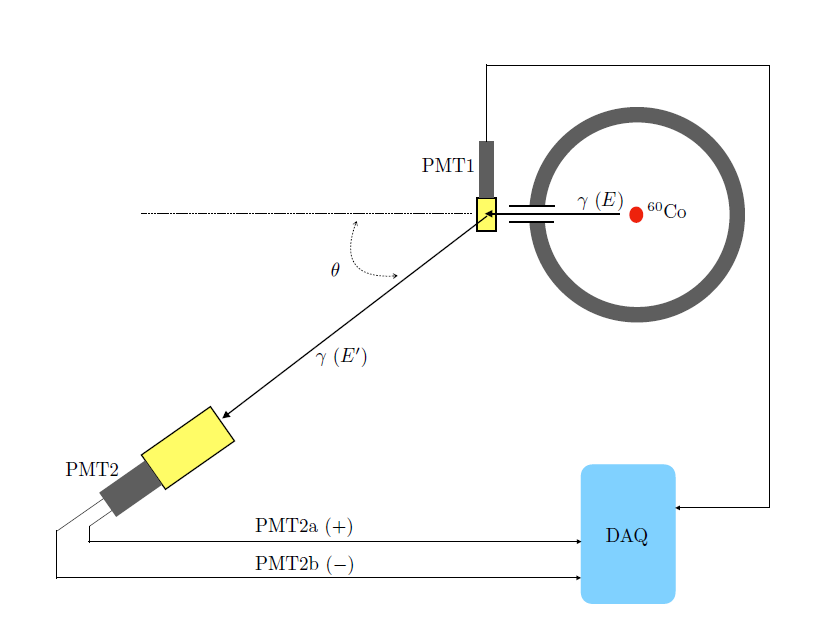
\includegraphics[width=\textwidth]{apparato}
	\caption{\label{fig:apparato}
	Apparato di misura.
	La struttura portante non è disegnata.
	La guida ottica e il tubo fotomoltiplicatore (PMT) sono disegnati solo per il PM6.}
\end{figure}

Abbiamo a disposizione 6 lastre di scintillatore plastico
posizionate orizzontali e allineate verticalmente,
che non possiamo spostare,
collegate a tubi fotomoltiplicatori (vedi \autoref{fig:apparato}).


\subsection{Obiettivo}
Lo scopo dell'esperienza é la misura della massa dell'elettrone sfruttando l'effetto Compton: fotoni di energia nota (prodotti da una sorgente di \co) fanno scattering su un bersaglio e uno spettrometro ne misura l'energia $E'$ ad un certo angolo di scattering $\theta$.

\subsection{Apparato di misura}
Gli strumenti principali a disposizione per questa esperienza (fatta eccezione per i soliti moduli \texttt{NIM}) consiste in:
\begin{itemize}
	\item una sorgente radioattiva principale di \co\! e altre sorgenti meno attive per la calibrazione: \cs, \na, \am;
	\item il PMT1: un rivelatore basato su uno scintillatore organico (che fungerà da bersaglio);
	\item il PMT2: un rivelatore basato su un cristallo scintillatore di NaI(Tl) $\SI2{''}\times\SI2{''}$ dotato di un preamplificatore in cascata al fotomoltiplicatore (che useremo come spettrometro);
	\item un formatore/amplificatore che produce in uscita un segnale gaussiano con altezza di picco proporzionale all'energia rilasciata e durata $\sim \SI{10}{\micro s}$;
	\item un ADC a 13 bit che può sia essere triggerata dall'esterno, sia campionare automaticamente sul picco tutti i segnali che superano una certa soglia interna (chiameremo questa modalità \emph{automatica}).
\end{itemize}

\subsubsection{Sorgenti radioattive}
La sorgente radioattiva principale di \co\; decade $\beta^-$ in uno stato eccitato di $^{60}$Ni che a sua volta decade $\gamma$ due volte in cascata emettendo fotoni di $\SI{1.17}{MeV}$ e $\SI{1.33}{MeV}$.

La sorgente ha un'attività dichiarata di \SI{74}{MBq} al febbraio 1997 e si trova in un contenitore di piombo con collimatore a sezione circolare\footnote{Di un materiale diverso e a Z più basso.}. 
Data l'emivita del \co\; di $\tau_2 = \SI{5.3}{yr}$ alla data della nostra esperienza l'attività stimata della sorgente è $\sim 2^{21/5.3} \cdot \SI{74}{MBq} = \SI{4.7}{MBq}$.

Dalla costante di dose del \co\;  ($\SI{0.37}{\micro Sv\;m^2\;MBq^{-1}\;h^{-1}}$, vedi \cite{1}) è possibile stimare la dose assorbita nel corso dell'esperienza: $\SI{0.37}{\micro Sv\;m^2\;MBq^{-1}\;h^{-1}} \cdot \SI{4.7}{MBq} \cdot (\SI{1}{m})^2= \SI{1.7}{\micro Sv\;h^{-1}}$ (a un metro di distanza) che va confrontato con il fondo naturale $\sim\SI{0.3}{\micro Sv\;h^{-1}}$. Si tratta di una stima per eccesso poiché considera la sorgente isotropa, ma la nostra sorgente è schermata ed emette solo in un piccolo angolo solido (non nella nostra direzione).

Le altre sorgenti di calibrazione a disposizione hanno un'attività minore di $\SI{72}{kBq}$\footnote{Si tratta dell'attività dichiarata dalla ditta produttrice alla data di vendita che è ignota.}\marginpar{questo dettaglio non è particolarmente rilevante ma bho (Bob)} e i loro principali modi di decadimento sono schematizzati in \autoref{tab:sorgenti_cal}. Notiamo inoltre che il \na\; decade $\beta^+$, ci aspettiamo perciò di osservare nel suo spettro il segnale dei fotoni $\gamma$ a \SI{511}{keV} prodotti nell'annichilazione.

\begin{table}[h]
	\centering
	\begin{tabular}{cccc}
		\toprule
		sorgenti & \multicolumn{3}{c}{principali modi di decadimento} \\
		\midrule
		\co & $\beta^{-} (\SI{318}{keV})$ & $\gamma (\SI{1173}{keV})$ & $\gamma (\SI{1332}{keV})$  \\
		\cs & $\beta^{-} (\SI{512}{keV})$ & $\gamma (\SI{662}{keV})$ \\
		\na & $\beta^{+} (\SI{546}{keV})$ & $\gamma (\SI{1275}{keV})$ \\
		\am & $\alpha (\SI{5486}{keV})$ & $\gamma (\SI{59.5}{keV})$ \\
		\bottomrule
	\end{tabular}
	\caption{\label{tab:sorgenti_cal} Principali modi di decadimento delle sorgenti a disposizione \cite{2}}
\end{table} 

\subsubsection{Schema dell'apparato sperimentale}
La strumentazione a disposizione è disposta come in \autoref{fig:schema_apparato}: il PMT1 si trova subito davanti al collimatore della sorgente di \co. Il PMT2 si trova su una base capace di ruotare attorno ad un perno (che con buona approssimazione si trova sulla verticale del bersaglio) e di variare la distanza dal bersaglio (in un range $\sim\SI{40}{cm}-\SI{20}{cm}$).
L'angolo di scattering ovvero l'angolo tra la direzione del fascio di fotoni primari e i fotoni secondi prodotti è misurato come mostrato in \autoref{fig:goniometro}: abbiamo stampato un goniometro su carta e e lo abbiamo sotto la base ruotante del PMT2 in modo che il centro fosse nel perno di rotazione che lo 0 fosse circa lungo la direzione del fascio primario. Una tacca sulla base trasparente ci consente di leggere l'angolo. Questa soluzione ci permette di misurare gli angoli con grande comodità e precisione (stimiamo di avere una risoluzione migliore di $\sfrac14 \si{\degree}$).

 \begin{figure}[h]
	\centering
	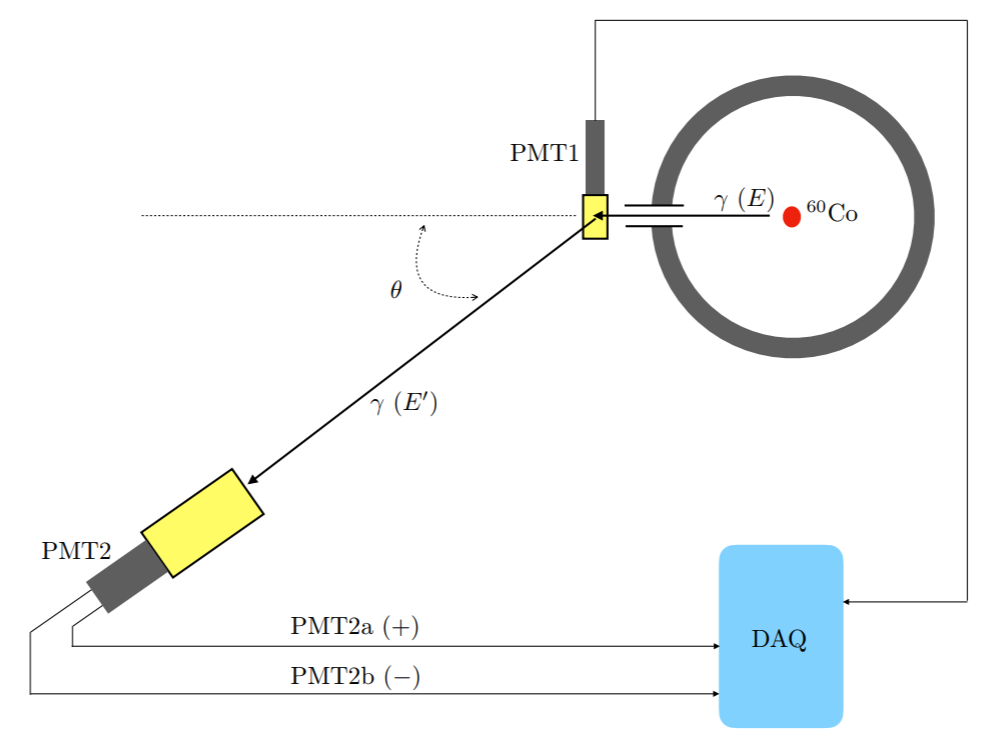
\includegraphics[width=25em]{schema_apparato}
	\caption{\label{fig:schema_apparato}Schema dell'apparato sperimentale.}
\end{figure}
 \begin{figure}[h]
	\centering
	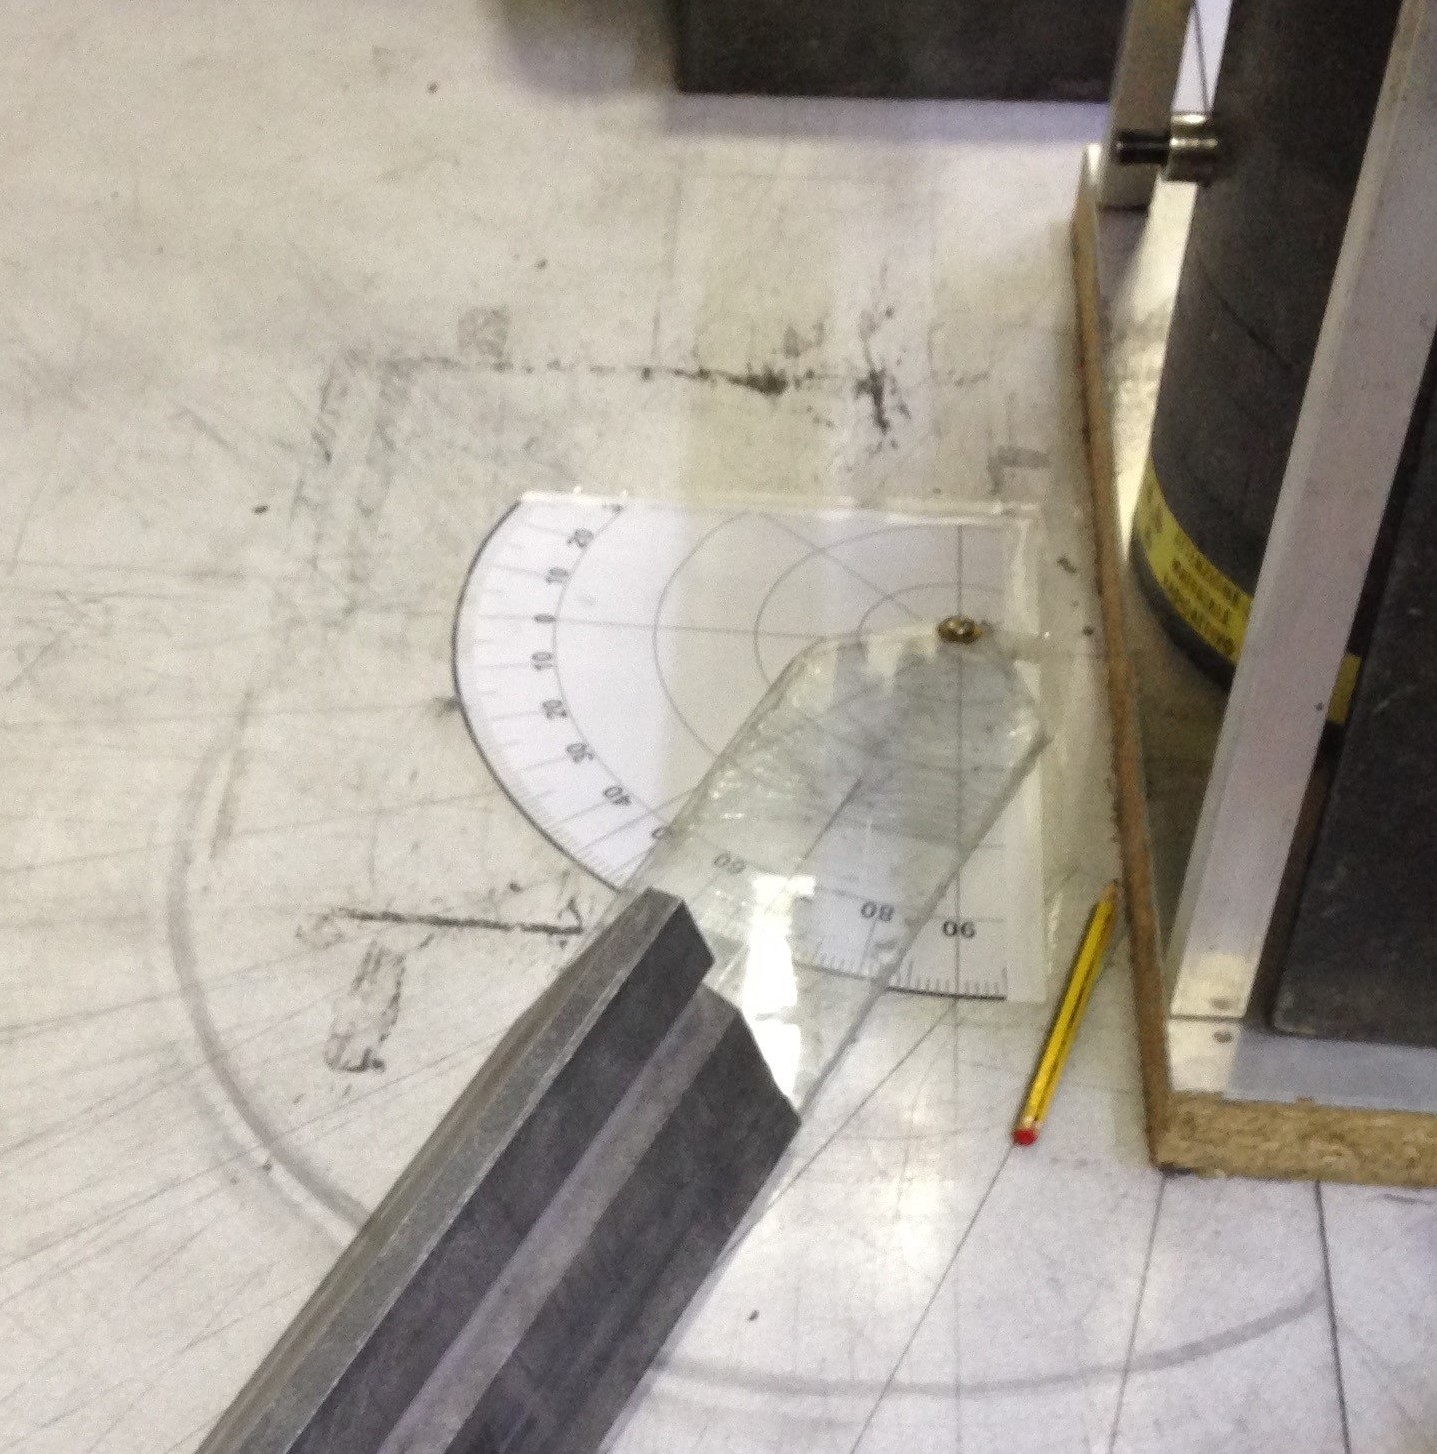
\includegraphics[width=15em]{goniometro}
	\caption{\label{fig:goniometro}Goniometro usato per la misura degli angoli.}
\end{figure}



\section{Teoria}

\subsection{Spettrometria $\gamma$}
Riassumiamo il principio di misura dell'energia del nostro spettrometro:
\begin{itemize}
	\item particelle cariche attraversano il cristallo scintillatore rilasciando energia all'interno per eccitazione/ionizzazione degli elettroni dello stesso;
	\item lo scintillatore produce luce in funzione dell'energia rilasciata ($\sim \SI{40}{fotoni \; keV^{-1}}$ nel NaI(Tl));
	\item i fotoni raggiungono il fotomoltiplicatore dopo essere stati riflessi sulle pareti del cristallo (rivestite di materiale riflettente) e nella guida ottica;
	\item il fotomoltiplicatore amplifica il segnale dei fotoni e produce in uscita un segnale (negativo e di breve durata: $\sim \SI{10}{\nano s}$) di picco proporzionale al numero di fotoni;
	\item la base del fotomoltiplicatore in dotazione fornisce anche un segnale pre-amplificato positivo a bassa impedenza (perciò di lunga durata $\sim \SI{1}{\micro s}$);
	\item questo segnale viene riconosciuto dal formatore/amplificatore che produce in uscita un segnale gaussiano di durata nota ($\SI{10}{\micro s}$) e di picco proporzionale all'energia rilasciata;
	\item l'output dell'amplificatore va all'ADC (tipicamente triggerato da un segnale esterno) che campiona sul massimo del segnale in una finestra temporale imposta dal trigger e converte il segnale in tensione in un segnale digitale a 13 bit.
\end{itemize}
Ciascuno di questi processi sarà caratterizzato da una:
\begin{itemize}
	\item\emph{funzione di risposta}: la funzione che da un certo input mi dà l'output medio (ad esempio energia della particella vs energia media rilasciata, energia rilasciata vs numero medio di fotoni prodotti, segnale in tensione vs digit, tutte in prima approssimazione lineari nel nostro range di lavoro\footnote{discuteremo nel seguito la validità di questa approssimazione});
    \item una \emph{distribuzione di risposta}: la distribuzione degli output a input fissato (ad esempio la distribuzione dei fotoni prodotti ad una energia fissata, queste ci aspettiamo avranno generalmente un forma a campana, in prima approssimazione gaussiana).
\end{itemize}
La misura finale avrà per funzione di risposta la composizione di tutte queste funzioni di risposta e per distribuzione di risposta la convoluzione delle distribuzioni di risposta (quest'ultima determinerà la risoluzione sperimentale).

Nella nostra esperienza lo spettrometro dovrà misurare l'energia di fotoni $\gamma$ che, essendo neutri, devono prima interagire con la materia del rivelatore e trasferire tutta o parte della loro energia a particelle cariche, delle quali sarà poi misurabile l'energia nel modo descritto sopra. Bisogna quindi analizzare le interazioni fotone-materia per modelizzare gli spettri che andremo poi ad osservare.

\subsubsection{Interazione fotone-materia}
I principali meccanismi di interazione dei fotoni con la materia sono:
\begin{itemize}
	\item assorbimento fotoelettrico;
	\item scattering Rayleigh;
	\item scattering Compton;
	\item produzione di coppie.
\end{itemize}
  
 \paragraph{Assorbimento fotoelettrico}
 Il fotone incidente è completamente assorbito e ionizza l'atomo, ovvero estrae un elettrone di energia cinetica $T_e = E_{\gamma} - E_b$, dove $E_{\gamma}$ è l'energia del fotone incidente e $E_b$ è l'energia di legame, solitamente piccola se paragonata a $E_{\gamma}$. Nel nostro caso l'energia di legame vale al massimo $\sim \SI{33}{keV}$ per gli elettroni 1s dello iodio, da confrontarsi con l'energia dei fotoni $\gamma$ del \co\;: \SI{1.17}{MeV} e \SI{1.33}{MeV}. Il risultato finale è una particella carica nello scintillatore con approssimativamente la stessa energia del fotone incidente.
 Un elettrone con energia cinetica di $\SI{1}{MeV}$ ha un range in NaI di $\sim \SI{2}{mm}$ FONTE CIPPA LIPPA, questo vuol dire che questi fotoni perdono tutta la loro energia nel nostro rivelatore (un cilindro retto $\sim \SI{5}{cm} \times \SI{5}{cm}$). 

 \paragraph{Scattering Rayleigh}
 Nello scattering Rayleigh l'intero atomo funge da bersaglio, perciò dopo l'urto il fotone cambia direzione e l'atomo rincula per conservare il momento. Data la grande massa dell'atomo (rispetto all'energia del fotone) l'energia scambiata è trascurabile e il fotone uscente ha praticamente la stessa energia iniziale. \`E chiaro quindi che i fotoni non potranno essere rivelati in uno scintillatore con questo meccanismo perché nessuna energia viene rilasciata all'interno.
 
 \paragraph{Scattering Compton}
 Se il fotone è abbastanza energetico può urtare un singolo elettrone. Per fotoni di questo tipo l'energia di legame può essere in prima approssimazione trascurata e si può trattare l'elettrone come libero. Nello stato finale troviamo il fotone che è stato deviato di un certo angolo $\theta$ rispetto alla sua direzione iniziale e ha ceduto parte della sua energia all'elettrone. La relazione tra energia del fotone dopo lo scattering e angolo è:
 \begin{equation}
 \label{energia_compton}
 E' = \frac{E}{1+\frac{E}{m_ec^2}(1-\cos(\theta))}   
 \end{equation}
 Quello che misureremo nello spettroscopio sarà l'energia ceduta all'elettrone cioè $E-E'$. Quando un fotone fa scattering Compton nel nostro spettroscopio non abbiamo modo di conoscere l'angolo di scattering e non è possibile da una singola misura ricavare l'energia del fotone incidente.
 La sezione d'urto differenziale di questo processo (anche nota come formula di Klein–Nishina) è:
 \begin{equation}
 \label{klein-nishina}
 \frac{d\sigma}{d\cos(\theta)} = \frac{\pi}{m_e^2} \cdot\left(\frac{E'}{E}\right)^2 \cdot \left(\frac{E}{E'} + \frac{E'}{E} - \sin^2(\theta)\right)
 \end{equation}
 dove $\frac{E'}{E}$ contiene implicitamente l'angolo: $\frac{E'}{E} = \frac{1}{E(1-\cos(\theta))/(m_ec)}$
 La sezione d'urto differenziale è graficata in \autoref{fig:klein-nishina} ed è da qui evidente come all'energia di $\sim \SI{1}{MeV}$ è molto più probabile che il fotone sia deviato poco.
 
 \begin{figure}[h]
 	\centering
 	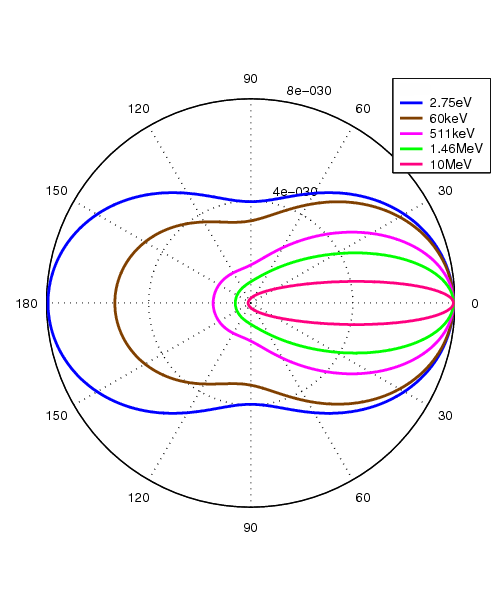
\includegraphics[width=16em]{klein-nishina}
 	\caption{\label{fig:klein-nishina}Sezione d'urto in funzione dell'angolo di scattering Compton}
 \end{figure}

 \paragraph{Produzione di coppie}
 Il fotone $\gamma$ può fare scattering con un fotone del campo e.m. del nucleo (o meno probabilmente di un elettrone) e produrre una coppia $e^+e^-$. Aaffinchè questo processo sia accessibile cinematicamente l'energia del fotone deve essere $> \SI{1.02}{MeV}$, quindi questo processo è possibile per i fotoni del \co\;  e del \na, tuttavia come vederemo questo processo è largamente trascurabile a queste energie, rispetto agli altri in gioco.
 
 \subsubsection{Sezione d'urto fotone-materia}
 La sezione d'urto fotone-materia per ciascuno dei processi prima descritti dipenderà dallo Z del materiale. In generale a basse energie ($ < \SI{10}{keV}$) sarà dominante l'assorbimento fotoelettrico, ad alte energie ($>\SI{100}{MeV}$) predominerà la produzione di coppie mentre lo scattering Compton sarà dominante in un range intermedio. L'estensione di questo range è maggiore al diminuire di Z come è chiaro dalla \autoref{fig:photon_cross_section_pdg}.
 
  \begin{figure}[h]
 	\centering
 	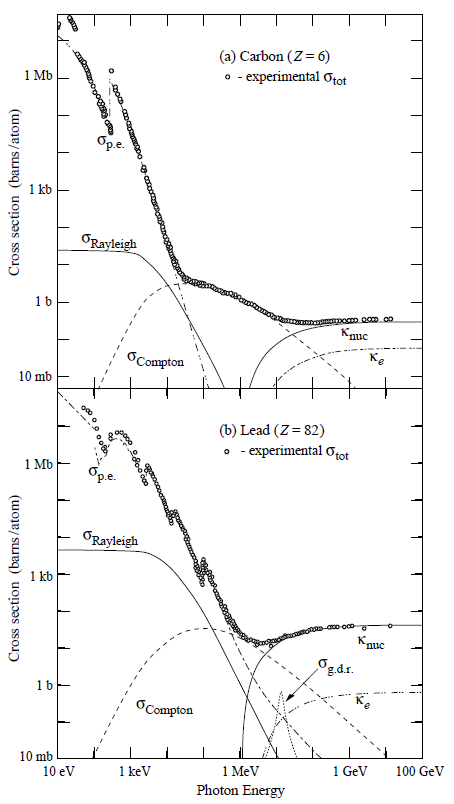
\includegraphics[width=16em]{cross_section_photon_pdg}
 	\caption{\label{fig:photon_cross_section_pdg}Sezione d'urto in funzione dell'energia per i vari processi nel carbonio e nel piombo FONTE CIPPLIPPA}
 \end{figure}

 \paragraph{Scelta del materiale per bersaglio e spettrometro}
 Nella nostra esperienza il bersaglio sarà di carbonio, mentre lo spettrometro è un cristallo di NaI ($\text{Z}(\text{Na})=11$, $\text{Z}(\text{I})=53$). Questa scelta è giustificata dal fatto che nel carbonio, all'energia dei fotoni del \co\; la sezione d'urto dell'assorbimento fotoelettrico è ampiamente trascurabile e l'energia del fotone è più facilmente misurabile dai fotopicchi associati all'assorbimento fotoelettrico. Sarà perciò preferibile usare il cristallo di NaI come spettrometro poichè a $\sim{1}{MeV}$ il rapporto tra sezione d'urto Compton e sezione d'urto dell'assorbimento fotoelettrico vale $\sim 20$, (come si può vedere anche in \autoref{fig:photon_cross_section_xcom})questo è sufficiente per rendere i fotopicchi chiaramente visibili con la risoluzione strumentale. Inoltre scegliendo il carbonio per il bersaglio  sarà garantito che tutti i fotoni che interagiranno nel carbonio lo faranno per effetto Compton.
 
  \begin{figure}[h]
 	\centering
 	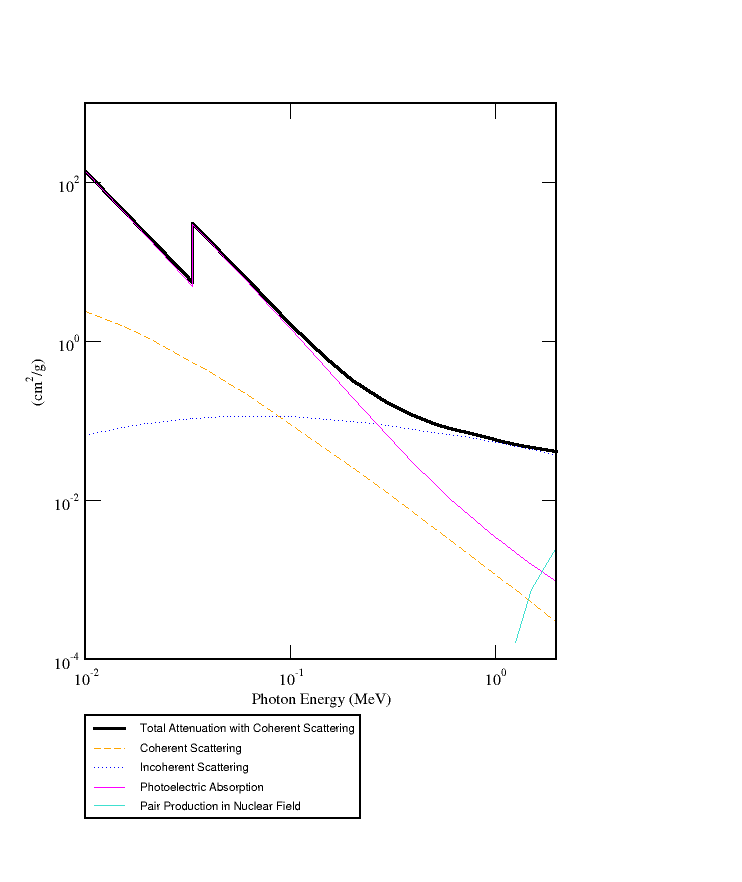
\includegraphics[width=28em]{photon_cross_section_xcom}
 	\caption{\label{fig:photon_cross_section_xcom}Sezione d'urto in funzione dell'energia per i vari processi nel NaI FONTE CIPPALIAPPA}
 \end{figure}
 
 \subsubsection{Risposta del detector}
 \paragraph{Grande detector} Se il detector fosse abbastanza esteso, tutta l'energia dei fotoni, indipendentemente dalla complessità dell'interazione, verrebbe rilasciata nel rivelatore. Per una sorgente di fotoni ad una energia fissata, come potrebbe essere una sorgente di raggi $\gamma$\footnote{I raggi $\gamma$ delle sorgenti radioattive hanno tipicamente larghezze $\Gamma \ll \SI{1}{eV}$ e possono quindi considerarsi mono-energetici per i nostri scopi.}, ad esempio il \cs, lo spettro energetico prodotto da un tale scintillatore sarebbe un singolo fotopicco all'energia dei fotoni $\gamma$ (vedi \autoref{fig.spettrometro_grosso} con una larghezza dovuta essenzialmente alla risoluzione dello strumento, come analizzeremo nel seguito.
 
 \begin{figure}[h]
 	\centering
 	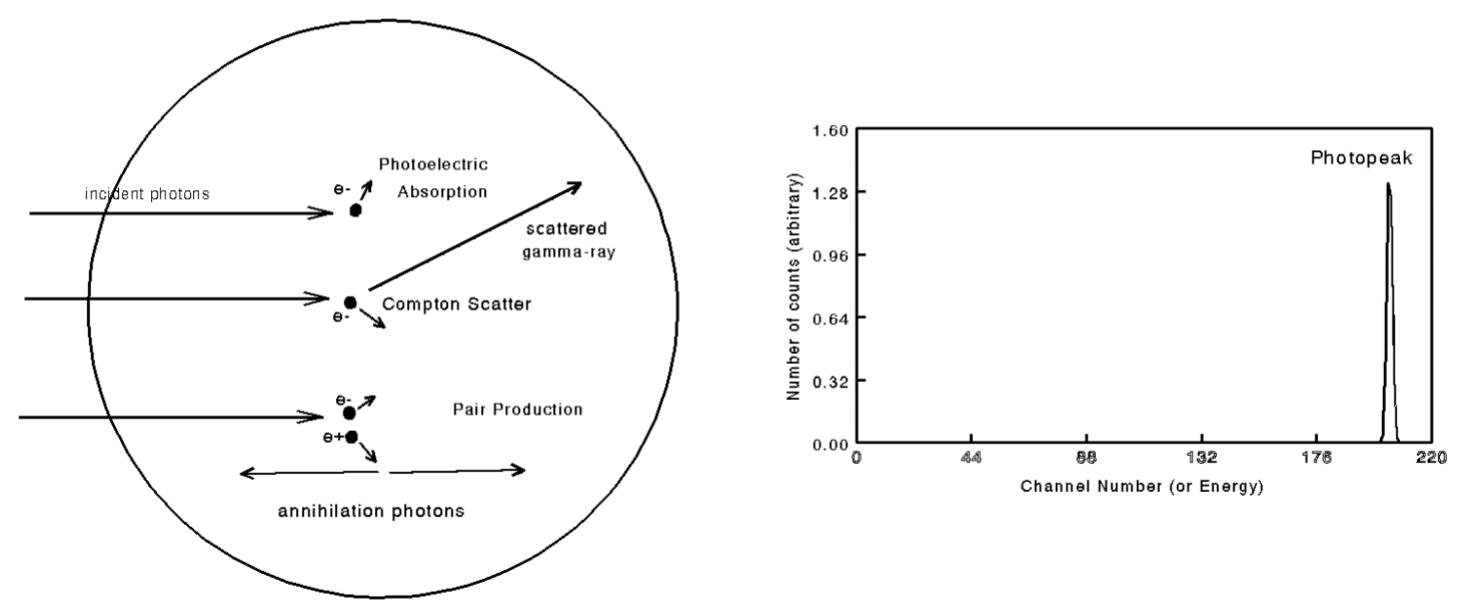
\includegraphics[width=28em]{spettrometro_grosso}
 	\caption{\label{fig:spettrometro_grsso}Risposta di un detector di grandi dimensioni per fotoni mono-energetici}
 \end{figure}

 \paragraph{Piccolo detector}Nel caso opposto di un detector di piccole dimensioni (e trascurando la produzione di coppie, per i motivi detti sopra) i fotoni potranno interagire una sola volta, facendo effetto fotoelettrico o Compton in proporzione alla sezione d'urto. I fotoni che fanno effetto fotoelettrico produrranno un segnale alla loro energia (che non sarà una delta ma sarà allargato dalla risoluzione strumentale) come visto prima, mentre i fotoni che faranno fotoelettrico si produrranno uno spettro come quello predetto dalla sezione d'urto di Klein-Nishina (la spalla Compton sarà meno definita perché convoluta con la risoluzione strumentale). Il risultato finale sarà simile a quelli in \autoref{spettrometro_piccolo}
 
  \begin{figure}[h]
 	\centering
 	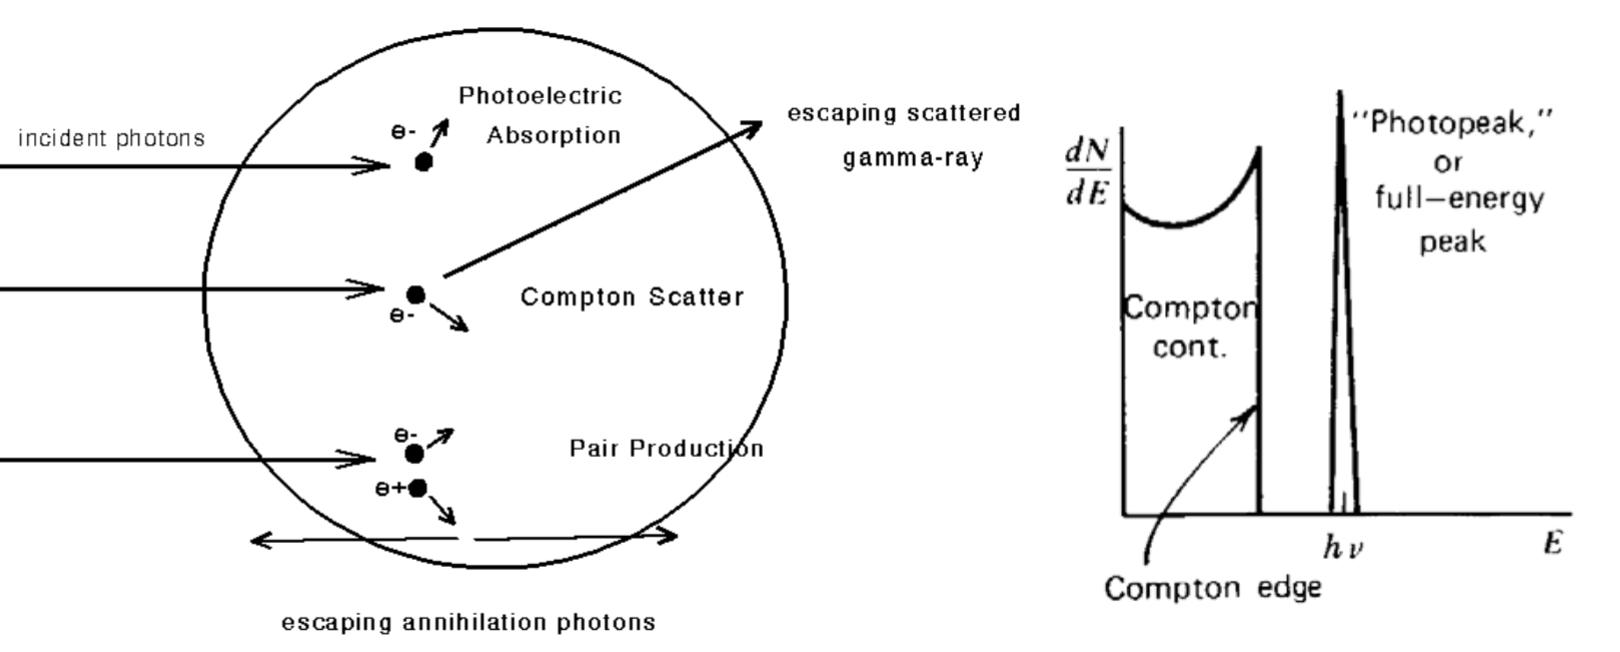
\includegraphics[width=28em]{spettrometro_piccolo}
 	\caption{\label{fig:spettrometro_piccolo}Risposta di un detector di piccole dimensioni per fotoni mono-energetici}
 \end{figure}
 
 \paragraph{Detector di dimensioni intermedie}Nel nostro caso disponiamo di un rivelatore $2"\times2"$ e, a partire dal grafico in FONTE che ci dà la lunghezza di radiazione al variare dell'energia del fotone in vari materiali, è semplice calcolare che per il nostro rivelatore la lunghezza di radiazione:$\sim \SI{5}{cm}$, quindi paragonabile alla dimensione del cristallo, ne segue che il $\sim 60\%$ dei fotoni interagisce nel cristallo. Ci troviamo quindi in una situazione intermedia per cui in pratica lo spettro sarà simile a quello in \autoref{spettrometro_piccolo}, ma il rapporto tra gli eventi Compton e quelli fotoelettrico non sarà uguale al rapporto tra le sezioni d'urto: è infatti importante il contributo di quei fotoni che dopo aver fatto Compton fanno fotoelettrico\footnote{Questo processo è favorito a basse energie e i fotoni perdono energia facendo Compton} (quando ancora si trovano nello spettrometro): questi finiranno nel fotopicco poiché tutta l'energia è rilasciata nello scintillatore. 
 
 Lo spettro finale prodotto sarà la somma di molti effetti:
 \begin{itemize}
 	\item l'assorbimento fotoelettrico produrrà un fotopicco all'energia dei fotoni incidenti;
 	\item i fotoni che fanno scattering Compton rilasceranno solo parte della loro energia producendo il caratteristico profilo predetto dalla  formula di Klein-Nishina;
 	\item i fotoni che fanno scattering Compton sui materiali che circondano il detector possono tornare nello stesso producendo un picco, detto di backscattering nella regione a basse energie;
 	\item spesso potrebbe essere visibile un picco all'energia caratteristica dei raggi X emessi dai materiali circostanti (ad esempio lo stesso spettrometro).
 \end{itemize}
  
 
 \subsubsection{Efficienza}
 
 \subsubsection{Linearità}
 Un rivelatore di radiazione ideale dovrebbe essere perfettamente lineare 
 \subsection{Risoluzione}
 
 
 
 
 

\subsection{Simulazione}

Implementiamo una simulazione Monte Carlo dello scattering Compton nel bersaglio
e della rivelazione nello spettrometro.
Ogni fotone è simulato in questo modo:
\begin{enumerate}
	\item Viene estratta una direzione iniziale da una gaussiana per tenere conto della larghezza del fascio.
	\item Viene simulato lo scattering Compton nel bersaglio,
	usando la formula \eqref{klein-nishina} per estrarre gli angoli e \eqref{energia_compton} per calcolare l'energia.
	Lo scattering avviene in un centro fissato (non teniamo conto della dimensione del bersaglio).
	\item Se il fotone passa per lo spettrometro,
	viene calcolata la probabilità che faccia Compton oppure fotoelettrico nel cristallo.
	L'energia rilasciata per il fotoelettrico è quella del fotone,
	per il Compton è quella cinetica dell'elettrone, trascurando l'energia di legame
	(non simuliamo che il fotone possa fare Compton più di una volta).
	\item Applichiamo la calibrazione da energia a scala dell'ADC.
	\item Aggiungiamo a ogni energia un'estrazione gaussiana
	per simulare la risoluzione.
\end{enumerate}
Gli spettri di fotoelettrico e Compton sono ottenuti con un istogramma pesato con le probabilità di interazione calcolate.
La normalizzazione relativa di fotoelettrico e Compton è macroscopicamente errata,
supponiamo perché non abbiamo tenuto conto dei fotoni che fanno Compton più di una volta,
quindi non la teniamo in considerazione.


\section{Misura e analisi}

\subsection{Misure e osservazioni preliminari}

\subsubsection{Punto di lavoro del PMT2}

Vogliamo trovare un buon punto di lavoro per il PMT2 che è alimentato con tensioni positive fino a $\sim \SI{800}{V}$. 
Mandiamo il segnale preamplificato del PMT2 all'amplificatore e la sua uscita all'ADC in modalità automatica.
Scegliamo di alimentare il PMT2 alla tensione consigliata di \SI{650}V. A questa tensione (e con guadagno dell'amplificatore impostato a $\times 1$) il fotopicco generato dai fotoni più energetici tra le sorgenti a disposizione (ovvero il picco a \SI{1.33}{MeV} del \co) si trova a $2/3$ della scala. Questo permette, agendo sul fattore di amplificazione del formatore/amplificatore di portare il fotopicco a fondo scala  e massimizzare la risoluzione dello spettrometro, mantenendo allo stesso tempo flessibilità nel caso la risposta del rivelatore non si rivelasse stabile\footnote{Cosa che abbiamo verificato essere vera: la posizione dei fotopicchi può variare nel tempo fino al $\sim 10\%$.}.

\subsubsection{Stabilità della risposta del PMT2}

Notiamo che la risposta dello spettrometro è molto sensibile alle variazioni della tensione di alimentazione:
variando da \SI{600}V a \SI{575}V, la posizione dei fotopicchi si dimezza.
Il manuale dell'alimentatore riporta una stabilità dello \SI{0.5}{\permil} su \SI{24}h e dell'\SI1{\permil} su un mese. Volendo fare una stima otteniamo variazioni del $2/25 \times 600/1000 = \SI5\%$ in un mese, la metà in \SI{24}h. Sembra quindi che la stabilità della risposta del nostro spettrometro sia un limite importante nella nostra misura per cui nel seguito analizzeremo approfonditamente questo parametro.
%%%%%%%%%%%%%%%%%%%%%%%%%%%%%%%%%%%%%%%%%%%%%%%%%%%%%%%%%%%

\subsubsection{Interazione con il bersaglio}

Poniamo lo scintillatore plastico (PMT1) davanti alla sorgente in modo che i raggi~$\gamma$ possano interagire e subire scattering Compton. Osserviamo l'istogramma dei campionamenti del nostro spettrometro a vari angoli rispetto al bersaglio (ne riportiamo due in \autoref{4ang}) mentre l'ADC campiona in modalità automatica.
Il range dei fotoni del \co\; nel bersaglio è $\sim\SI{10}{cm}$ e il suo spessore $\sim\SI{1}{cm}$, quindi solo il $10\%$ dei fotoni interagisce. 
Se lo spettrometro si trova a piccolo angolo rispetto al bersaglio viene attraversato dai fotoni che non hanno interagito e lo spettro è sostanzialmente uguale a quello acquisito senza bersaglio. A grande angolo vorremmo vedere i fotoni che fanno Compton sul bersaglio e arrivano con un certo angolo di scattering sul rivelatore (producendo quindi uno spettro simile al precedente ma traslato a energie minori) ma i fotoni che non interagiscono proseguono sino al muro subito dietro lo spettrometro, una parte di questi fa scattering Compton o Rayleigh e può arrivare nello spettrometro, sovrastando in statistica il segnale che vorremmo osservare.

\begin{figure}[h]
	\centering
	\newcommand*\mywidth{0.5\textwidth}

	\subfloat
	{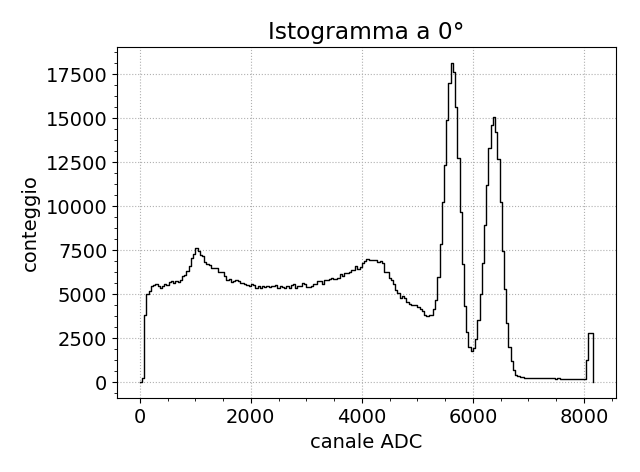
\includegraphics[width=\mywidth]{0g}}
	\hfill
	\subfloat
	{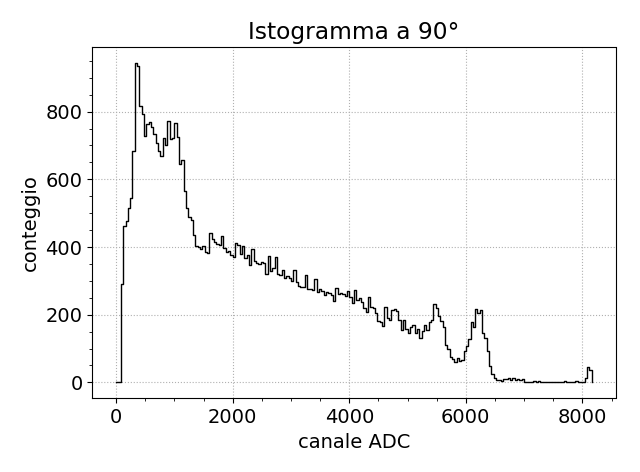
\includegraphics[width=\mywidth]{90g}}

	\caption{Spettri raccolti senza coincidenza a diversi angoli rispetto al bersaglio.}
	\label{4ang}
\end{figure}

Abbiamo poi confrontato lo spettro a \SI{45}{\degree} con o senza scintillatore plastico, ma non abbiamo notato nessuna differenza. Abbiamo anche verificato che, come atteso, il rate di eventi diminuisce all'aumentare della distanza.

Proviamo a schermare lateralmente lo scintillatore cristallino per ridurre il fondo di backscattering e lo spettro in \autoref{casetta} mostra come effettivamente questo si riduca ma non a sufficienza da poter osservare il segnale. Si rende necessario l'uso di un trigger esterno per campionare sulla coincidenza di segnale tra PMT1 e PMT2.

\begin{figure}
\centering

\subfloat{
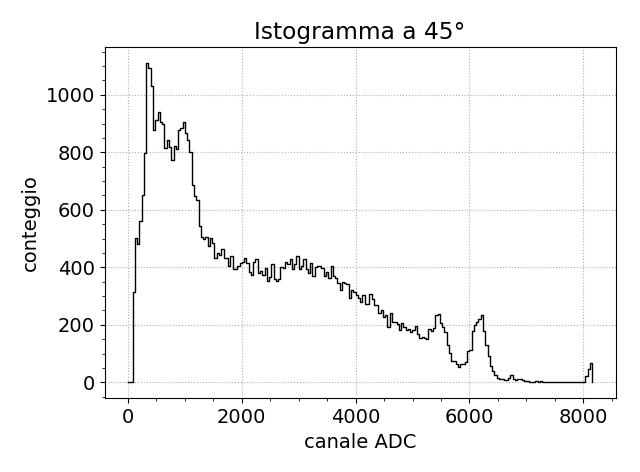
\includegraphics[width=0.5\textwidth]{45g} }
\subfloat{
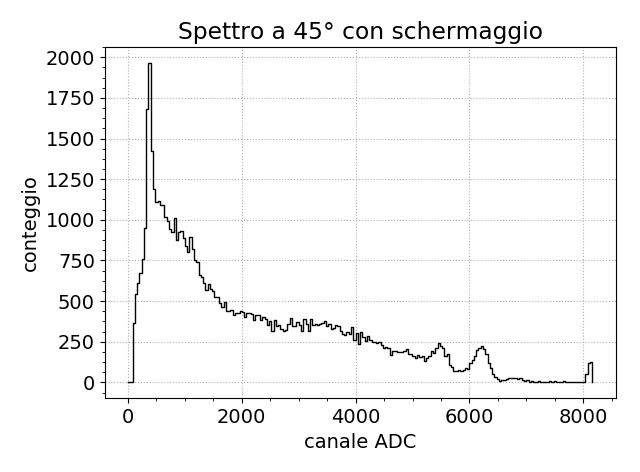
\includegraphics[width=0.5\textwidth]{45gs} }

\caption{Confronto tra gli spettri a 45$^{\circ}$ con e senza schermaggio.}
\label{casetta}
\end{figure}

\subsubsection{Trigger esterno}
Per ottenere il segnale di trigger usiamo il circuito in \autoref{fig:trigger}:\marginpar{aggiungere figura?(Bob)}
\begin{itemize}
	\item il segnale ``veloce'' del PMT2 (quello non pre-amplificato con ampiezza di picco $\sim\SI{20}{mV}$) è prima amplificata di un fattore 10 attraverso un modulo di amplificazione lineare, quindi inviato ad un discriminatore con soglia a $\SI{35}{mV}$ (il minimo) in modo da ottenere una soglia efficace più bassa;
	\item il segnale del PMT1 è inviato direttamente ad un discriminatore con soglia a $\SI{35}{mV}$ (il minimo);
	\item entrambi gli output dei discriminatori vanno ad un sistema di anti-rettriger che impone un tempo morto di $\sim\SI{1}{\micro s}$ e produce segnali di durata $\sim\SI{30}{ns}$;
	\item il segnale discriminato del PMT1 è ritardato di circa \SI{20}{ns} per compensare un ritardo asimmetrico dovuto al modulo di anti-retrigger;
	\item facciamo la coincidenza dei due segnali così formati e mandiamo l'output a un modulo \texttt{gate \& delay}.
	\item l'ADC richiede un segnale di trigger che parta almeno \SI{200}{ns} prima del picco e termini almeno \SI{200}{ns} dopo: usando l'oscilloscopio, regoliamo il modulo \texttt{gate \& delay} in modo da avere un segnale della durata di $\sim\SI{1}{\micro s}$ centrato sul picco del formatore.
\end{itemize}
Acquisiamo degli spettri di prova e verifichiamo che con le soglie impostate i primi $\sim1000$ canali dell'ADC non mostrano campionamenti.

\subsubsection{Punto di lavoro del PMT1}
Il PMT1 può essere alimentato fino a \SI{1800}{V} e nel range \SI{1500}{V}-\SI{1700}{V} mostra circa lo stesso rate. Decidiamo di alimentarlo a \SI{1700}{V} per avere alta efficienza e mantenendo il rate ragionevole.
\marginpar{tenerlo lontano da 1800\! V non conta niente? \\ (Andrea)}

\subsubsection{Stabilità della risposta del PMT2}



\subsection{Misure in coincidenza}

Per misurare soltanto l'energia dei fotoni che hanno subito diffusione Compton, realizziamo una coincidenza temporale tra i due PMT. Sappiamo che il PMT1 deve avere un'alimentazione inferiore ai \SI{1800}V; facendo varie prove notiamo che il rate di coincidenze tra \SI{1500}V e \SI{1800}V rimane circa invariato. Impostiamo allora la tensione di alimentazione del PMT1 a \SI{1700}V in modo da avere un'alta efficienza ed essere lontani da zone in cui il dispositivo è malfunzionante.
\marginpar{Ho letto dal logbook che questo lo abbiamo fatto dopo, ma penso che mentire a favore del filo logico non ci nuocia in questo caso.\\
Forse dobbiamo parlare dei pocci con l'attenuatore  e dei retrigger.}

Il circuito di misura è stato poi ottimizzato e segue lo schema di \autoref{sc_conc}. Il segnale positivo del PMT2 è rimasto collegato al formatore come nelle misure precedenti \autoref{???} 

%\begin{thebibliography}{99} % Bibliography

\bibitem[1] {1}
Laurie M. Unger, D. K. Trubey, Specific gamma-ray dose constants for nuclides important to dosimetry and radiological assessment, ORNL/RSIC-45/RI, \emph{Oak Ridge National Laboratory} (1982).

\bibitem[2] {2}
S.Y.F. Chu, L.P. Ekström, R.B. Firestone, The Lund/LBNL Nuclear Data Search Version 2.0, \emph{Berkeley National Laboratory} (1999).

\bibitem[3]{3}
M.J. Berger, J.S. Coursey, M.A. Zucker, J. Chang, Stopping-power \& range tables for electrons, protons, and helium ions, \emph{National Institute of Standards and Technology} (2017).

\bibitem[4]{4}
K.A. Olive et al., Passage of particles through matter, (PDG), Chin. Phys. C38, 090001 (2014).

\bibitem[5]{5}
M.J. Berger, J.H. Hubbell, S.M. Seltzer, J. Chang, J.S. Coursey, R. Sukumar, D.S. Zucker, and K. Olsen, XCOM: Photon Cross Sections Database XCOM, \emph{National Institute of Standards and Technology} (2010).

\bibitem[6]{6}
G.F. Knoll, Radiation Detection and Measurement- 3rd edition (Capitolo 10), \emph{Wiley} (1999).

\bibitem[7]{7}
P. M. Bergstrom Jr, Compton scattering of photons from electrons bound in light elements, \emph{Argonne National Laboratory} (1994).

\bibitem[8]{8}
P.M. Bergstrom Jr, R.H. Pratt, An overview of the theories used in Compton scattering calculation, \emph{Radiat. Phys. Chem.} Vol. 50, No. 1, pp. 3-29 (1997).

\end{thebibliography}


\end{document}